\documentclass{article}
\usepackage{hyperref}
\usepackage{listings}
\usepackage{color}
\usepackage{xcolor}
\usepackage{geometry}
\usepackage{graphicx}
\usepackage{amsmath}
\usepackage{caption}
\usepackage{subcaption}
\geometry{margin=1in}
\pdfminorversion=6

\newcommand\TODO[1]{\textcolor{red}{TODO: #1}}

\newcommand\header[2]{
    \begin{center}
        {\large
        UCSD CSE 168 Assignment #1: \\
        \vspace{0.3cm}
        \Large
        #2}
    \end{center}
}

\definecolor{dkgreen}{rgb}{0,0.6,0}
\definecolor{gray}{rgb}{0.5,0.5,0.5}
\definecolor{mauve}{rgb}{0.58,0,0.82}
\lstset{frame=tb,
        aboveskip=3mm,
        belowskip=3mm,
        showstringspaces=false,
        columns=flexible,
        basicstyle={\small\ttfamily},
        numbers=none,
        numberstyle=\tiny\color{gray},
        keywordstyle=\color{blue},
        commentstyle=\color{dkgreen},
        stringstyle=\color{mauve},
        breaklines=true,
        breakatwhitespace=true,
        tabsize=2
}

\hypersetup{colorlinks=true}


\begin{document}

\header{1}{Ray Tracing}
\setcounter{section}{-1}

In our first homework, we are going to implement a simple ray tracer (almost) from scratch.
We will provide some utility code such as the vector class and parallel threading. 
However, you will have to implement the rest yourself. Trust me, it will be fun!

Our homeworks are mostly inspired by the book \href{https://raytracing.github.io/}{Ray Tracing in One Weekend (RTOW)} (click the link for free access of the e-book). You are expected to read the relevant chapters of the book before implementing your own version. The structure of the homeworks is also largely inspired by \href{https://cs87-dartmouth.github.io/Fall2022/assignments.html}{CS 87/287 at Dartmouth} designed by Wojciech Jarosz (a UCSD alumni!).

Before you started coding, we recommend you to go through the whole handout to have some ideas of what needs to be done.

\paragraph{Coordinate systems conventions.} This is the most annoying part of any graphics systems as every single one of them use a different one. We will follow the conventions used in RTOW: Y axis is up, negative Z looks into the screen from the viewer, and we use a right-handed coordinate system.

\paragraph{Links in this document.} Some of the links in this document contain hyperlinks with a \emph{named anchor} to a webpage (e.g., \url{https://raytracing.github.io/books/RayTracingInOneWeekend.html\#overview}). On some PDF readers, I have found these links to not work very well (Adobe Acrobat Reader works well). If you encounter issues with the links, try replacing \lstinline{%23} with \lstinline{#} in the address bar of your browser.

\section{Building Torrey}
We are going to build our code on top of (a currently very barebone) renderer \emph{torrey}. Torrey already includes all the third party libraries (pugixml, pcg, stb\_image, tinyexr, miniz, tinyply) in its repo and all you need to do is to clone the repo and build it using CMake (assuming you are in a Unix-like system):
\begin{lstlisting}[language=bash]
  git clone https://github.com/BachiLi/torrey_public
  mkdir build
  cd build
  cmake ..
  make -j
\end{lstlisting}

After building, you should see an executable \lstinline{torrey}. Try typing the following command:
\begin{lstlisting}[language=bash]
  torrey -hw 1_1
\end{lstlisting}
It will generate an image \lstinline{hw_1_1.exr} that looks like the following:
\begin{figure}[h]
    \centering
    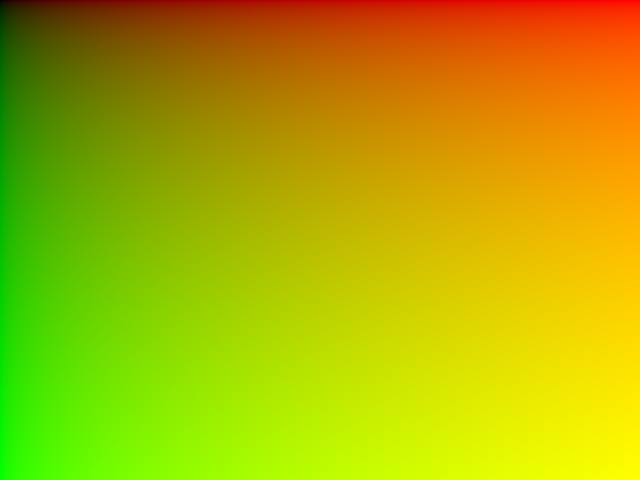
\includegraphics[width=0.5\linewidth]{imgs/hw_1_1_before.png}
    \caption{Image output by the homework 1.1 code before your modification.}
    \label{fig:hw_1_1_before}
\end{figure}

\lstinline{.exr} is an image format that is suitable for storing \emph{high-dynamic range} images. Basically, instead of storing 8-bit (0-255) per color channel, we store a floating point number per channel. To view \lstinline{.exr}, I recommend using \href{https://github.com/wkjarosz/hdrview}{HDRView} or \href{https://github.com/Tom94/tev}{Tev}.

Read \lstinline{main.cpp}, \lstinline{hw1.cpp}, \lstinline{vector.h}, and \lstinline{image.h} to understand the current code structure.

\section{Sending rays from the camera}
To do ray tracing, we need to first shoot rays from the camera. In this first step, we will generate camera rays for all the pixels. The goal of our first task is to visualize the camera ray direction (normalized to unit length per pixel).

First, read \href{https://raytracing.github.io/books/RayTracingInOneWeekend.html\#rays,asimplecamera,andbackground}{Chapter 4.2} of the first RTOW book and understand its content.

We will use a very simple perspective camera for now. The position is fixed at $(0, 0, 0)$, and the camera is facing towards $(0, 0, -1)$ with an up vector $(0, 1, 0)$, right vector $(1, 0, 0)$, and focal length of $1$. We will make the camera ``positionable'' later. For each pixel, we will shoot a ray from the center of the pixel (for a pixel $(x, y) \in [0, \text{width}] \times [0, \text{height}]$, we shoot a ray in $(x + 0.5, y + 0.5)$). Go to \lstinline{hw1.cpp} and look at the function \lstinline{hw_1_1}. Your task is to modify the function to output the \emph{unit length} ray direction per pixel. Some of the pixels will have negative color but that is fine. We provide the \lstinline{.exr} image we generated from our code for your reference.

Don't worry about the \lstinline{params} argument of the function. We will use it in the later part.

To see your results, in terminal, type
\begin{lstlisting}[language=bash]
  torrey -hw 1_1
\end{lstlisting}

\begin{figure}[h]
    \centering
    
\includegraphics[width=0.5\linewidth]{imgs/hw_1_1_after.png}
    \caption{Image output by the homework 1.1 code after your modification.}
    \label{fig:hw_1_1_after}
\end{figure}

\paragraph{Quiz:} How do you modify your code to render using a camera with 360 degree field of view like the following image? (hint: see \href{https://en.wikipedia.org/wiki/Spherical_coordinate_system}{spherical coordinates}) Briefly describe your approach or attach your code.
\begin{figure}[h]
    \centering
    \includegraphics[width=0.5\linewidth]{imgs/360camera.png}
    \caption{360 camera rendering taken from the \href{https://www.pbr-book.org/3ed-2018/Camera_Models/Environment_Camera}{PBRT book}.}
    \label{fig:360_camera}
\end{figure}

\section{Intersection with one sphere}
After we have the rays from the camera, we'll trace these rays and intersect them with the scene. Here we choose the geometry to be a sphere (because it's easy and we can easily build interesting scenes using only spheres). For this part, let's try to handle only one sphere.

First, read \href{https://raytracing.github.io/books/RayTracingInOneWeekend.html\#addingasphere}{Chapter 5} and \href{https://raytracing.github.io/books/RayTracingInOneWeekend.html\#surfacenormalsandmultipleobjects}{Chapter 6} of RTOW and understand the content.

Next, go to \lstinline{hw1.cpp} and look at the function \lstinline{hw_1_2}. Your task is to modify the function to output the surface normal of the sphere. The sphere has unit radius and is located at $(0, 0, 2)$. The camera pose is exactly the same as the previous part. To avoid negative number this time, let's map the normal to positive numbers: for a 3D vector $n$, we map it to the final color $c = \frac{n + 1}{2}$.

You may find the struct \lstinline{SpherePrimitive} in \lstinline{hw1_scenes.h} to be helpful, but you are not required to use it.

To see your results, in terminal, type
\begin{lstlisting}[language=bash]
  torrey -hw 1_2
\end{lstlisting}

The results generated from our code looks like this:
\begin{figure}[h]
    \centering
    \includegraphics[width=0.5\linewidth]{imgs/hw_1_2.png}
    \caption{Your homework 1.2 should output this image.}
    \label{fig:hw_1_2}
\end{figure}

\paragraph{Quiz:} If we were to add a linear transformation to the sphere (e.g., turn it into an ellipsoid), how would you do it?

\section{Adding camera control}
We will next add pose and field of view control to the camera so that we can look at the sphere at different angles. We will adopt the LookAt transform since it's more intuitive. We will also follow RTOW and take a vertical field of view angle.

First, read \href{https://raytracing.github.io/books/RayTracingInOneWeekend.html#positionablecamera}{Chapter 11} of RTOW and understand the content.

Next, go to \lstinline{hw1.cpp} and look at the function \lstinline{hw_1_3}. Given the inputs \lstinline{lookfrom}, \lstinline{lookat}, \lstinline{up}, \lstinline{vfov} (we have parsed it for you), transform your camera rays accordingly and render the same sphere in \lstinline{hw_1_2}.

\section{Intersection with many spheres}
Next, we will extend our ray tracer to handle multiple spheres in the scene. Take your code from the previous part, and add a for loop to intersect with all the spheres. This part should be much easier than the previous one. 

Go to \lstinline{hw1.cpp} and modify the function \lstinline{hw_1_3}. We will use the command line argument \lstinline{params} to access the scenes. Use \lstinline{hw1_scenes[scene_id]} to access your scene. The scene is contained in the struct \lstinline{HW1Scene}:
\begin{lstlisting}[language=C++]
struct HW1Scene {
    std::vector<SpherePrimitive> primitives;
    std::vector<PointLight> lights; 
};
\end{lstlisting}
Ignore the lights for now. We will use the lights later.
After you intersect the spheres, instead of outputting the normal, we will output the \lstinline{diffuse_color} of the sphere this time.

To see your results, in terminal, type
\begin{lstlisting}[language=bash]
  torrey -hw 1_3 [scene_id]
\end{lstlisting}
where \lstinline{[scene_id]} is the scene you want to render (0-3).

%\bibliographystyle{plain}
%\bibliography{refs}

\end{document}
